\documentclass[11pt,a4paper]{article}
\usepackage[margin=2.5cm]{geometry}
\usepackage[T1]{fontenc}
\usepackage{lmodern}
\usepackage{microtype}
\usepackage{graphicx}
\usepackage{booktabs}
\usepackage{amsmath}
\usepackage[numbers]{natbib}
\PassOptionsToPackage{hyphens}{url}
\usepackage[hidelinks]{hyperref}
\urlstyle{tt}
\graphicspath{{../../output/figures/}}

\title{BTP Progress Report --- Part 3}
\author{Devansh Gupta}
\date{1 November 2026}

\begin{document}
\maketitle

\section{Scope of Part 3}
Part 3 covers Tasks 8 to 11 of the implementation plan. Task 8 is the R descriptive analysis. Task 9 is the Makefile and the clean-clone rebuild check. Task 10 is the structure of the BTP-I report. Task 11 is the Beamer slides.
Part 3 builds on the Git tag \texttt{part2}.

\section{What was built}
\subsection{R descriptive functions and script}
The file \path{src/R/lib/descriptives_fns.R} has three functions. \texttt{main\_sample} keeps the rows with \path{in_main_sample} true. \texttt{sigma\_cv} gives the coefficient of variation (standard deviation with $n-1$, divided by the mean) across the main-sample states for each period. \texttt{beta\_convergence} fits an ordinary least squares regression of annualised growth on the logarithm of the initial level.
The script \path{src/R/01_descriptives.R} reads \path{data/final/panel_quarterly.csv} and writes the outputs below. The tests are in \path{tests/R/test_descriptives.R}.
The figures in \path{output/figures/} are:
\begin{itemize}
\item \path{adoption_trend_main.pdf}: median and interquartile range of ln(real value per person), by quarter.
\item \path{sigma_convergence.pdf}: the coefficient of variation by quarter.
\item \path{adoption_map_2018Q4.pdf}: state map for 2018Q4.
\item \path{adoption_map_2026Q2.pdf}: state map for 2026Q2.
\end{itemize}
The tables in \path{output/tables/} are:
\begin{itemize}
\item \path{summary_stats.tex}: summary statistics.
\item \path{beta_convergence.tex}: the two beta regressions (Section~\ref{sec:beta}).
\item \path{validation_npci.tex}: the PhonePe against NPCI correlations.
\end{itemize}
% Command: ls output/figures output/tables   (output: 4 PDF files; summary_stats.tex beta_convergence.tex validation_npci.tex)

\subsection{Makefile and clean-clone rebuild check}
The \path{Makefile} has the targets \texttt{all}, \texttt{test}, \texttt{data}, \texttt{analysis} and \texttt{report}. \texttt{test} runs pytest and the R tests. \texttt{data} runs the Python modules from the raw-data check to the NPCI validation. \texttt{analysis} runs \path{src/R/01_descriptives.R}. \texttt{report} builds the report, the slides and the progress reports with latexmk.
% Command: grep -E "^[a-z]+:|^\.PHONY" Makefile   (output: .PHONY: all test data analysis report; all: test data analysis report)
The rebuild check was run in a clean clone of the repository. The outputs of the clone were compared byte for byte with the outputs of the working tree. The compared files are the CSV files in \path{data/final}, \path{data/interim} and \path{data/manual}, and the files in \path{output/tables}. All compared files are identical. The figure PDFs are not compared. Each PDF has a creation date inside the file.
% Source of the rebuild result: controller record for Task 9. This command was not run again in Part 3.

\subsection{Report structure}
The BTP-I report is \path{thesis/btp1/main.tex}. It has six chapters: Introduction, Literature Review, Data, Methodology, Preliminary results, and Plan for BTP-II. The student writes the prose of the chapters.
% Command: grep -n "chapter{" thesis/btp1/chapters/*.tex   (output: ch1 Introduction; ch2 Literature Review; ch3 Data; ch4 Methodology; ch5 Preliminary results; ch6 Plan for BTP-II)

\subsection{Slides}
The slides are \path{thesis/btp1-slides/slides.tex}. The file has 14 frames.
% Command: grep -c '\\begin{frame}' thesis/btp1-slides/slides.tex   (output: 14)
% Command: pdfinfo thesis/btp1-slides/slides.pdf | grep Pages   (output: 15; the PDF has 15 pages)
The PDF has 15 pages.

\section{Numbers}
\subsection{Beta convergence}\label{sec:beta}
The sample is the main sample (30 states and union territories), 2018Q4 to 2026Q2. For each state, growth is $(\ln x_{2026Q2} - \ln x_{2018Q4})/7.5$. The regression is growth on $\ln x_{2018Q4}$ with an intercept (OLS). The standard errors are the classical OLS standard errors.
% Command: .venv/bin/python -c "import pandas as pd, numpy as np; p=pd.read_csv('data/final/panel_quarterly.csv'); m=p[p.in_main_sample]
%   for v in ['real_amount_pc','count_pc']: w=m.pivot(index='state_id',columns='period',values=v); x=np.log(w['2018Q4']); y=(np.log(w['2026Q2'])-x)/7.5; X=np.c_[np.ones(30),x]; b=np.linalg.lstsq(X,y,rcond=None)[0]; r=y-X@b; se=np.sqrt(r@r/28*np.linalg.inv(X.T@X).diagonal()); print(v,b,se,1-r@r/((y-y.mean())@(y-y.mean())))"
%   (output: real_amount_pc slope 0.0174 se 0.0138 intercept 0.3773 se 0.0788 R2 0.054 N 30; count_pc slope -0.0030 se 0.0128 intercept 0.5751 se 0.0211 R2 0.002 N 30; same values as output/tables/beta_convergence.tex)
\begin{table}[h]
\centering
\caption{Beta regressions, main sample, 2018Q4 to 2026Q2. Dependent variable: annualised growth of the variable.}
\begin{tabular}{lrr}
\toprule
 & Real value per person & Transactions per person \\
\midrule
Slope on ln(initial level) & 0.0174 & $-0.0030$ \\
Standard error & 0.0138 & 0.0128 \\
$R^2$ & 0.054 & 0.002 \\
$N$ & 30 & 30 \\
\bottomrule
\end{tabular}
\end{table}
The slope for real value per person is positive (0.0174, standard error 0.0138). The slope for transactions per person is negative ($-0.0030$, standard error 0.0128). Neither slope is more than 1.3 standard errors from zero.
% Command: python3 -c "print(0.0174/0.0138, 0.0030/0.0128)"   (output: 1.26 0.23)

\subsection{Coefficient of variation}
The coefficient of variation (CV) is the sample standard deviation divided by the mean, across the 30 main-sample states.
% Command: .venv/bin/python -c "import pandas as pd; p=pd.read_csv('data/final/panel_quarterly.csv'); m=p[p.in_main_sample]
%   for v in ['count_pc','real_amount_pc','users_per_1000']: print(v, [round(m[m.period==q][v].std(ddof=1)/m[m.period==q][v].mean(),3) for q in ['2018Q4','2026Q2']])"
%   (output: count_pc [0.854, 0.865]; real_amount_pc [0.719, 0.906]; users_per_1000 [0.622, 0.379])
\begin{table}[h]
\centering
\caption{Coefficient of variation across the 30 main-sample states.}
\begin{tabular}{lrr}
\toprule
Variable & 2018Q4 & 2026Q2 \\
\midrule
Transactions per person & 0.854 & 0.865 \\
Real value per person & 0.719 & 0.906 \\
Registered users per 1000 persons & 0.622 & 0.379 \\
\bottomrule
\end{tabular}
\end{table}
The CV of real value per person rose from 0.719 to 0.906. The CV of transactions per person rose from 0.854 to 0.865. The CV of registered users per 1000 persons fell from 0.622 to 0.379.

\subsection{Tests}
% Command: .venv/bin/pytest -q   (output: 83 passed)
% Command: Rscript -e 'testthat::test_dir("tests/R")'   (output: [ FAIL 0 | WARN 0 | SKIP 0 | PASS 2 ]; grep -c test_that tests/R/test_descriptives.R gives 2)
The command \path{.venv/bin/pytest -q} reports 83 passed. The R command \path{testthat::test_dir("tests/R")} reports 0 failures, 0 warnings, 0 skipped and 2 passed expectations. The file \path{tests/R/test_descriptives.R} has 2 \texttt{test\_that} blocks.

\subsection{Report length}
% Command: make report; pdfinfo thesis/btp1/main.pdf | grep Pages   (output: 17)
The command \path{pdfinfo thesis/btp1/main.pdf} reports 17 pages after \texttt{make report}.

\begin{figure}[h]
\centering
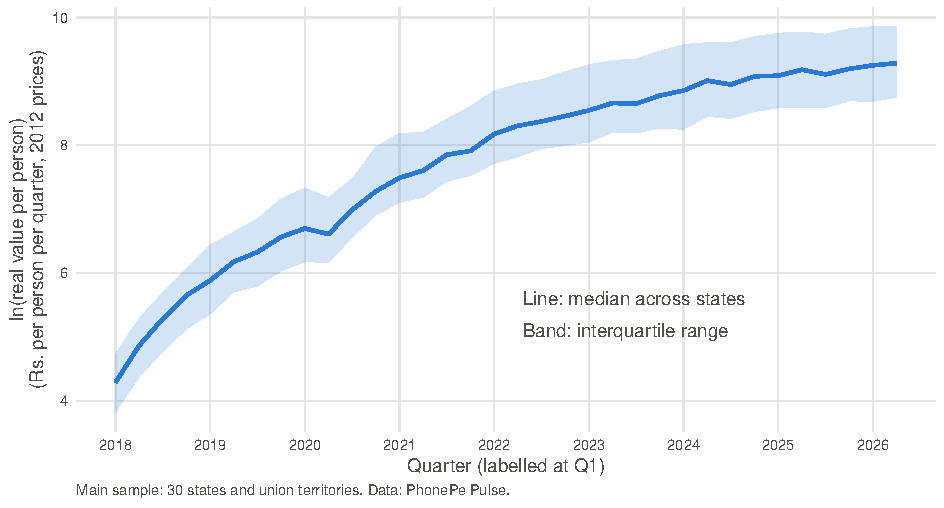
\includegraphics[width=0.8\textwidth]{adoption_trend_main.pdf}
\caption{Median (line) and interquartile range (band) of the natural logarithm of real value per person (Rs. per person per quarter, 2012 prices), by quarter, 2018Q1 to 2026Q2. Sample: 30 main-sample states and union territories. Source: PhonePe Pulse \citep{phonepe_pulse}; deflator: linked state CPI \citep{mospi_cpi}.}
\end{figure}

\section{Data notes for the thesis}
% Command: .venv/bin/python -c "import pandas as pd, json; p=pd.read_csv('data/final/panel_quarterly.csv'); q=p[p.period=='2026Q2']; t=q[q.state_id=='telangana'].iloc[0]; print(t.real_amount_pc, t.phonepe_amount_inr, t.phonepe_amount_inr/q.phonepe_amount_inr.sum(), t.population/q.population.sum(), len(q), q.phonepe_amount_inr.sum())
%   d=json.load(open('data/raw/phonepe/repo/data/map/transaction/hover/country/india/2026/2.json'))['data']['hoverDataList']; tot=sum(e['metric'][0]['amount'] for e in d); tel=[e for e in d if e['name']=='telangana'][0]['metric'][0]['amount']; print(len(d), tot, tel, tel/tot)"
%   (output: 61997.31 5.128e12 0.1127 0.0271 35 4.5496e13; JSON: 36 entries, total 4.5496e13, Telangana 5.128e12, share 0.1127)
In 2026Q2, the real value per person in Telangana is 61,997 Rs. (2012 prices).
Telangana has 11.3\% of the PhonePe transaction amount. The amount is Rs.\ $5.13\times10^{12}$ of Rs.\ $4.55\times10^{13}$. The PhonePe file for 2026 quarter 2 and the panel give the same total and the same share. Telangana has 2.7\% of the population of the 35 ids (38,664,500 persons).
% Command: .venv/bin/python -c "import pandas as pd; p=pd.read_csv('data/final/panel_quarterly.csv'); q=p[p.period=='2026Q2']; print(q[q.state_id=='telangana'].population.iloc[0])"   (output: 38664500.0)

\section{Open items}
\begin{itemize}
\item Task 0: supervisor approval of the PhonePe proxy. Department rules for BTP-I.
\item The student writes the prose of the report chapters.
\item The file \path{references/refs.bib} has four entries with a \texttt{verify} field:
\begin{itemize}
\item \path{pradhan2021tfsc}: ``verify exact title and full author list''.
\item \path{pradhan2021ael}: ``verify exact title and second author's given name''.
\item \path{reddy2024icrier}: ``year not shown on page, verify''.
\item \path{singh2021eap}: ``verify authors' given names''.
\end{itemize}
% Command: grep -n "verify " references/refs.bib | grep -v "^[0-9]*:%"   (output: lines 16, 28, 39, 50)
\item The open items of Part 2 stay open.
\end{itemize}

\section{Next}
BTP-II (Section 6, ``After BTP-I'', of the design specification) has these parts: financial inclusion data and indices, Steps 1 to 3 of the analysis, and the thesis. It also has a check with a district panel.

\bibliographystyle{plainnat}
\bibliography{../../references/refs}
\end{document}
